%------------------------------------------------- BiBliographie -------------------------------------------------%
	
	\part{Étude bibliographique}
	\parttoc
	
	\setcounter{chapter}{0} % Pour recommencer la numérotation des chapitres à 1
	\setcounter{section}{0} % Pour recommencer la numérotation des section à 1
	
	\renewcommand*{\theHchapter}{\thepart.\thechapter}
	\chapter{Transcription automatique d'un fichier audio vers un fichier texte}
	\section{Principe de fonctionnement de la reconnaissance automatique de la parole}
	La reconnaissance de la parole (RAP) est une forme de reconnaissance de forme, et suit donc le même type de procédure~\cite{invited-paper}. Ce dernier commence par la capture d'un signal correspondant au signal entrant enregistré par un locuteur lorsque celui-ci parle dans un microphone. Ces données sont par la suite compressées. Cette étape est primordiale pour pouvoir, d'une part travailler dans des temps raisonnables et d'autre part, permettre au processus de reconnaissance de se concentrer sur les aspects pertinent du signal. En effet, il est inutile de garder toutes les données, puisque beaucoup d'entre elles sont inutiles pour la RAP. Cependant, c'est aussi une étape très sensible, car une mauvaise compression peut également amener à perdre des informations primordiales au bon fonctionnement de la RAP. Vient ensuite la recherche de caractéristique dans le signal. On cherche ainsi à trouver un modèle ce rapprochant au maximum de ces caractéristiques. Enfin, il faut prendre une décision sur le modèle qui minimise au mieux et le coût, et les erreurs. 
	
	\section{Difficultés de l'analyse de la parole}
	De nombreux obstacles s'opposent à une bonne reconnaissance automatique de la parole.
	\subsection{Décompositions de la paroles en phonèmes}
	\subsubsection{Qu'est ce qu'un phonème ?}
	La parole est une succession de sons, que l'on identifie comme étant des phonèmes. Un phonème est en fait la plus petite unité d'un mot : un mot est constitué de syllabes, qui sont elles même constituées de phonèmes. Par exemple le mot "être" est constitué d'une seule syllabe, en revanche, il est constitué de trois voir quatre phonème (dépendant du fait que le locuteur prononce le 'e' final ou pas). Ces phonèmes sont représentés entre slash, de la même manière que les symboles de phonétique. Dans notre exemple nous avons donc les phonèmes suivant : \textipa{/E/}, \textipa{/t/}, \textipa{/r/} et éventuellement \textipa{/e/} .
	
	Le contenu basique de la parole est donc une séquence de phonèmes, qui une fois décodés, sont traduit par une séquence de mot grâce à une correspondance dans un dictionnaire.
	\subsubsection{Caractéristiques des phonèmes}
	Les phonèmes sont caractérisé par trois paramètres :
	\begin{itemize}
		\item{le mode d'articulation}
		\item{la place de l'articulation}
		\item{la voix}
	\end{itemize}
	Cependant par la suite, nous ne nous intéresserons dans le cadre de la RAP qu'au mode d'articulation.
	
	Le mode d'articulation correspond au type de son, que nous pouvons classer en 5 groupes majeurs :
	\begin{itemize}
		\item{Consonne occlusive : elle fait intervenir un blocage complet de l'air, suivit d'un relâchement soudain (i.e. /p,t,k,b,d,g/)}
		\item{Consonne fricative : l'air passe par une fente, formée par le rapprochement des lèvres, des dents, et/ou de la langue avec les lèvres/dents (i.e. /f,s,v,z/)}
		\item{Consonne nasale : il y a blocage complet, mais à l'inverse d'une consonne occlusive, l'air passe par le nez (i.e. /m,n/)}
		\item{Voyelles : pas d'obstruction de l'air, seule l'emplacement et la forme de la langue et des lèvres modifient le son}
		\item{Consonne latérale (ou liquide) et semi-voyelle : le premier correspond aux consonnes pour lesquelles l'air s'échappe par les côtés de la langue, et le second, aux lettres qui donne un son voyelle, mais sont pourtant caractérisées comme étant des consonnes(i.e. /l,r,w,j/)}
	\end{itemize}
	Il est ici important de rappeler que nous nous intéressons au type de son formé, et non à une lettre. Par exemple, ici la lettre 'c' n'est pas référencée, puisqu'elle se rapporte à deux sons : le son /k/ (e.g. dans le mot "caractère") et le son /s/ (e.g. dans le mot "ceci"). De la même manière, pour le groupe des sons voyelles, il ne faut pas se restreindre aux six voyelles de la langue française, puisque bien d'autres sons de type voyelle existent (e.g. \textipa{/\oe/} dans "oeuf", \textipa{/E/} dans "lait").
	
	Les systèmes de RAP n'ont pas de grandes difficultés à classer ces groupes de phonèmes, tout du moins lorsqu'il s'agit des groupes de consonnes occlusives, fricatives et de voyelles. En effet, ces sons ont de fortes caractéristiques, notamment une forte énergie périodique. Or ceci est une information primordiale car la détection de périodes est un facteur majeur de la RAP.
	
	
	
	\subsubsection{La coarticulation}
	Un phonème isolé est assez facile à identifier pour un système de RAP. Seulement, lorsque nous parlons, nous ne saccadons pas nos paroles en son. Nous enchainons les phonème, les mots, les uns après les autres, d'une manière plus ou moins fluide. C'est dans ce contexte qu'apparaît le principe de coarticulation.
	
	Un phonème intervient de façon significative sur le phonème qui le suit, mais également sur le phonème qui le précède. En effet, l'appareil vocal humain est fait de telle manière qu'il est impossible de passer d'un phonème à un autre (i.e. d'un son à un autre) instantanément. Pour chaque enchainement de phonèmes, il y a un moment de transition (plus ou moins importante et plus ou moins détectable). Pendant celle-ci, la forme des lèvres et la position de la langue et de la mâchoire vont se modifier, pour correspondre au prochain phonème. Par exemple, pour passer d'un son /s/ à un son /t/, la transition est le moment où l'on commence à avancer la langue jusqu'à ce que celle-ci touche les dents. Bien que difficilement détectable pour l'oreille humaine, cette transition apparait très clairement en terme de signal.
	
	De plus, dans la langue française, les règles de grammaires veulent que nous fassions les liaisons entres les mots, faisant ainsi apparaître des phonèmes.
	
	Ces deux phénomènes de coarticulation et de liaisons rendent la RAP très complexe, puisque un dictionnaire va associer à un mot les phonèmes qui le composent, et non les transitions. Ces transitions ne sont pas identifiables en terme de phonème et sont différentes pour chaque personne (vitesse de parole, appareil vocale différent, etc...). Il faut donc que le système de RAP apprennent à ne pas prendre en compte ces transitions. La liaison quant à elle est un tout autre problème, car elle fait apparaître des phonèmes tout à fait identifiable, "modifiant" ainsi les mots. C'est donc une nouvelle contrainte qui s'ajoute pour la RAP. Il est en effet parfois difficile de distinguer ces liaisons comme étant réellement des liaisons, e.g. "on en" et "on n'en". Nous pouvons en déduire qu'une reconnaissance simple des phonèmes n'est pas suffisante pour une bonne RAP : il faut y associer toutes les règles de grammaire de la langue.
	
	
	\subsection{Variabilité de la parole}
	Beaucoup de variabilité dans l'aspects de la parole peuvent intervenir et ainsi perturber la RAP~\cite{speech-variability}
	\begin{itemize}
		\item la physiologie de chaque individu : chacun individu est unique, et il en va de même pour son appareil vocal. En conséquence, chaque son produit par un individu est unique. Il faut donc un système de RAP suffisamment performant pour réussir à trouver une ressemblance dans un même phonème prononcé par différente personne.
		\item Les accents étrangers et régionaux : la langue d'origine influe inévitablement sur la prononciation, ainsi un espagnol par exemple aura tendance à rouler ses 'r' en français, ce qui change le phonème, créant une séquence de phonème qui ne peut pas être associé à un mot. De la même manière, pour les accents régionaux, bien que la langue reconnue est leur langue d'origine, ces individus ont un accent qui vient également changer certains phonèmes, et qui vient même en rajouter (e.g. l'accent marseillais). Pour ce cas, il faut un système qui soit capable de repérer que tel ou tel individu à tendance à prononcer ces phonèmes de telle manière.
		\item La vitesse de parole : tout le monde parle à sa vitesse, et cela complique d'avantage une bonne RAP, puisqu'entre deux individus, un qui parle lentement, et le second qui parle vite, la longueur des phonèmes varie énormément.
		\item L'état émotionnel : nous sommes humains, nous avons donc toute une panoplie d'émotions qui peuvent faire varier notre parole. Une personne en colère a tendance à parler fort et vite, supprimant ainsi certains phonèmes. Une personne sous pressions, stressée, a la gorge serrée, ce qui modifie les phonèmes.
		\item etc.
	\end{itemize}
	
	On voit donc ici que beaucoup d'élément peuvent venir perturber la RAP, même pour une unique personne. Suivant les instants, cette personne peut parler plus ou moins vite, se mettre en colère, etc... Si l'on y rajoute une personne avec un accent, qui est elle même sujette à toutes ces variations, on se rend compte de l'extreme complexité pour établir un bon système de RAP.
	
	
	
	\section{Variantes du problème de la reconnaissance de la parole}
	
	\subsection{Locuteurs connu et inconnu}
	Il existe deux types majeurs de systèmes de RAP :
	\begin{itemize}
		\item Locuteur connu
		\item Locuteur inconnu
	\end{itemize}
	
	\subsubsection{Locuteur connu}
	Ce type de système est le plus répandu, car il est le plus facile à réaliser. Il requiert une période d'entrainement (i.e. de réglage) pendant laquelle il lit des phrase à voix haute des phrases que lui indique le logiciel. Ainsi, ce dernier apprend la manière de parler de l'utilisateur. Il possède une base de données de phrase (qui sont choisies pour leur diversité de phonèmes), et sachant ce que l'utilisateur va dire, il peut associer chaque son à sa signification.
	
	\subsubsection{Locuteur inconnu}
	Ce deuxième type de système, quant à lui, est immédiatement opérationnel. Il ne requiert aucune période d'entrainement, et apprend seul, au fur et à mesure que l'utilisateur parle, à identifier ses phonèmes.
	
	\subsubsection{Analyse}
	Lorsque l'utilisateur est connu, le système donne souvent de bien meilleur résultat. Cependant, il présente un inconvénient majeur : une importante perte de temps pour l'utilisateur. De plus, son principe même a de fortes lacunes. En effet, ce type de système fait \textbf{lire} l'utilisateur alors que pendant son utilisation, les chances sont grandes que le locuteur parle spontanément plutôt que ne lise. Cependant, il est montré qu'en terme de signal, les phrases lues et les phrases parlées spontanément sont complètement différentes~\cite{read-spontaneous}.  La spontanéité demande plus de réflexion, et il plus d'émotion lorsque nous parlons que lorsque nous lisons. De plus, lorsque nous parlons spontanément, l'espace spectral se réduit, et plus la parole est spontanée, plus la réduction est importante (comme le montre la figure \ref{reduction_rate_phoneme_read_spontaneous}). Or une réduction de l'espace spectral provoque une réduction de la précision de reconnaissance de phonème, ce qui implique une réduction de la RAP.
	
	\begin{figure}[H]
		\begin{center}
			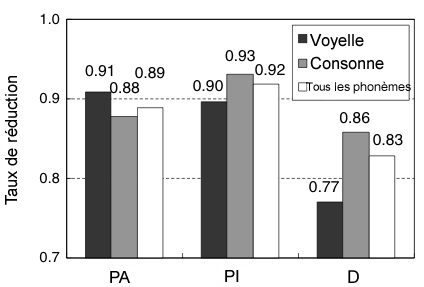
\includegraphics[width=10cm]{reduction_rate_phoneme_read_spontaneous}
			\caption{Moyenne du taux de réduction des voyelles, consonnes et tous les phonèmes pour les types PA, PI et D de paroles, respectivement Présentation Académique, Présentation Improvisée et Discours, par rapport à des phrases lues. \cite{read-spontaneous}}
			\label{reduction_rate_phoneme_read_spontaneous}
		\end{center}
	\end{figure}
	
	\subsection{Vocabulaire connu et limité ou vocabulaire large}
	Pour certains systèmes, le besoin de vocabulaire est très limité, et le système en perd en complexité. Par exemple, les répondeurs à reconnaissance automatique de la parole ne demandent que très peu de mots : "oui", "non", "suivant", "supprimer"... Il sont donc beaucoup plus facile à coder, puisque la suite de phonème ne correspond qu'à un mot, et les possibilités sont très rapides à parcourir.
	
	En l'occurrence, notre projet requiert un vocabulaire très large, puisqu'il doit pouvoir identifier tous les mots qui peuvent survenir lors d'une conversation entre différentes personnes. Cependant, même avec un vocabulaire extrêmement complet, il arrive couramment que des mots inconnus soient prononcés (e.g. nom propres, jargon scientifique, etc.)~\cite{retrieval-browsing-spoken-content}, et si un mot n'est pas dans le dictionnaire, alors la transcription sera forcément fausse. Pour palier à ce problème, plusieurs solutions existent. La première consiste à proposer à l'utilisateur plusieurs hypothèses, avec la possibilité d'ajouter un mot (i.e. de la même façon qu'il est possible d'ajouter des mots aux correcteurs orthographiques de logiciels de bureautique). Néanmoins, cette solution n'est pas envisageable pour notre projet, car ces vidéos seront faites lors de réunions professionnelles, et il n'est donc pas possible d'interrompre l'utilisateur pour chaque mot que le logiciel n'arrive pas à identifier. La deuxième solution, quant à elle, propose de rechercher les mots inconnus dans les documents associés à la vidéo. Cette dernière semble tout à fait appropriée à notre projet, puisqu'il est prévu que pour chaque réunion (i.e. visio-conférence) lui soit associé en plus de la vidéo et de l'audio, les documents utilisés lors de cette dernière. Il serait donc possible de parcourir ces documents afin d'éventuellement trouver le mot correspondant. Cependant, cette proposition ne peut pas fonctionner systématiquement, puisque d'une part, il n'est pas obligatoire que des documents aient été utilisés lors de la réunion, et d'autre part, quand bien même des documents auraient été partagés, les mots inconnus ne sont pas forcément contenu dans ces documents. Pour ce problème, nous pouvons proposer une troisième solution, qui consiste à faire une première passe du contenu parlé avec un tout autre système pour essayer d'en retirer le sujet de la vidéo, et ainsi créer un vocabulaire spécifique à ce sujet. Cette solution pourrait éventuellement faire l'objet d'une amélioration future par l'entreprise, mais elle ne sera pas employée pour notre projet.
	
	
	\subsection{Découpage temporel en locuteurs}
	Lorsque plusieurs locuteurs sont présents, il est intéressant de découper le flux de paroles en locuteurs. En effet, un bon modèle s'adapte au locuteur, or si nous ne différencions pas les différents locuteurs, le style de parole changeant à chaque prise de parole, il sera impossible au système de s'adapter convenablement. Ainsi, en découpant en locuteur, le système peut avoir plusieurs "adaptation" pour correspondre à chacun des locuteurs.
	
	Il n'est pas prévu de mettre cette fonctionnalité dans le projet pour l'instant, puisque nous partons du point de vue qu'il n'y a qu'un seul individu de chaque côté des micros. Dans ce contexte, la division est très simple, puisqu'une entrée correspond à un locuteur. Cependant, à terme, il doit être possible d'avoir plus d'une personne pour un micro, il y a donc une chance que l'entreprise nous demande d'inclure cette fonctionnalité.
	
	\subsection{Qualité acoustique de la composante parole}
	La précision de la RAP peut très vite chuter si la qualité audio est mauvaise, notamment s'il y a des bruits de fond~\cite{noisy-speech-recognition}, de la musique, une mauvaise transmission, etc.
	
	
	
	
	\chapter{Recherche d'information dans des documents parlés}
	\section{Son intérêt}
	L'augmentation constante de l'activité informatique et la réduction des coûts de stockage conduisent à un très fort nombre de données de tout types, échangées et stockées. En conséquence, la recherche de données est devenue un domaine clé, tout particulièrement celui de la recherche de données textuelles, qui est le plus courant~\cite{retrieval-browsing-spoken-content}.
	
	La recherche de document parlé, quant à elle, ne s'est pas beaucoup développée au fil des années, notamment dû à son manque de demande et d'exactitude. Cependant, dans les dernières année, l'explosion de contenu audio/vidéo disponible sur internet en fait un important outil. Néanmoins, ce domaine a nécessite encore beaucoup de progrès, car les résultats ne sont pas à la hauteur des exigences des utilisateurs. En effet, l'idéal serait de faire la recherche dans une transcription alignée avec l'audio, ce qui simplifierait le problème en une recherche textuelle. Malheureusement, dans cette hypothèse, le texte devrait être une transcription exacte de l'audio, ce qui nécessiterait une transcription manuelle. Or cette dernière prend du temps, et donc coûte cher. C'est dans ce contexte qu'intervient la recherche d'information des documents parlés.
	
	\section{Sa difficulté}
	Lorsque l'on crée un système de RAP pour une recherche d'information, le choix du dictionnaire est primordial. En effet, en général, le vocabulaire d'un ASR est assez restreint. Or, si un mot est prononcé et n'est pas dans le dictionnaire, alors le système de RAP de le reconnaitra jamais correctement, et les requêtes d'utilisateur contenant ce(s) mot(s) échoueront systématiquement. Malheureusement, les mots ou groupes de mots recherchés sont souvent les moins courants et les plus spécifiques à un sujet, qui ne sont généralement pas présent dans les dictionnaires des systèmes de RAP.
	
	On en déduit l'importance d'un système de recherche flexible, qui accepte des solutions avec des mots plus ou moins proches.
	
	\section{Différentes méthodes}
	La méthode la plus classique est évidemment une recherche textuelle classique dans les transcriptions des vidéos. Cependant, une autre méthode suggère d'attaquer le problème sous un autre angle, en ignorant totalement le texte, et de ne s'intéresser qu'à la prononciation. Le système de RAP, à la place de produire un texte de mots, produirait un texte de prononciation phonétique. La requête de l'utilisateur serait ensuite traduite en langage phonétique, et recherchée dans les transcriptions. Le très grand avantage de cette méthode est que solutionne le problème de vocabulaire inconnu. De plus, le système de RAP serait nettement plus performant puisqu'il n'aurait qu'à traduire ce qu'il "entend" en phonétique, et non plus à rechercher de correspondance dans son dictionnaire. En revanche, la recherche de mots clés, quant à elle, serait beaucoup plus longue. Or dans notre cas actuelle, la performance du système de RAP n'a pas de réelle importance puisqu'elle se fait en tache de fond, contrairement à la recherche qui se fait en temps réel.
	
	Une seconde solution utilise les deux méthodes précédentes, combinant à la fois la recherche par mot et la recherche phonétique. L'idée serait de faire une première recherche large (i.e très flexible quant à l'exactitude de la correspondance des mots) en utilisant les mots de l'utilisateur. Viendrait ensuite une seconde passe sur ces résultats, en utilisant la phonétique. Cette méthode impliquerait donc que le système de RAP produise deux transcriptions : une textuelle et une phonétique. Cela ne pose pas de réelle contrainte, puisque comme dit précédemment, la rapidité du système RAP n'a pas d'importance. La recherche, elle, serait plus rapide qu'avec la méthode n'utilisant que la phonétique, puisqu'ici elle ne se fait que sur un nombre de documents préalablement restreint.
	
	
	
	
	
	

	
	
	
	
	
	
	
	
	
	
	
		
	\nocite{introduction-hmm}
	\nocite{tutorial-hmm}
	